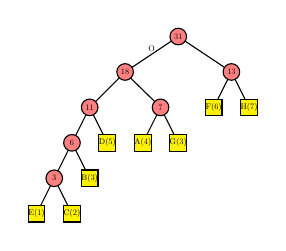
\begin{tikzpicture}[iv/.style={draw,fill=red!50,circle,minimum size=20pt,inner
    sep=0pt,text=black},ev/.style={draw,fill=yellow,rectangle,minimum
    size=20pt,inner sep=0pt,text=black},scale=0.3, every node/.style={transform shape}]
    \node[iv]{31}
      child {node[iv]{18}
             child {node[iv]{11}  
                    child {node[iv]{6}
                           child {node[iv]{3}
                                  child {node[ev]{E(1)}}
                                  child {node[ev]{C(2)}}
                                 }
                           child {node[ev]{B(3)}}
                          }
                    child {node[ev]{D(5)}}
                    }
             child [missing]
             child {node[iv]{7}
             child {node[ev]{A(4)}}
             child {node[ev]{G(3)}}
                   }
            edge from parent node[above]{O}        
            }
      child [missing]
      child [missing]
      child {node[iv]{13}
             child {node[ev]{F(6)}}
             child {node[ev]{H(7)}}
            };
\end{tikzpicture}